\setchapterpreamble[u]{\margintoc}
\chapter{Methodology}
\labch{method}

%---------------------------------------------------------------
% overview of chapter 
In this chapter, we describe the basic numerical methodology behind modeling 
the dynamics of immiscible incompressible liquid-gas interfacial flows under isothermal conditions. 
These implementations are developed on the platforms 'PARIS Simulator' \cite{paris} and 
'Basilisk' \cite{basilisk}, with considerable overlap between the two platforms in terms 
of the treatment of the interface capturing schemes, transport of conserved quantities and surface tension models.
\sidenote{The principle difference between 'PARIS Simulator' and 'Basilisk' is the ability to resolve the conservation
laws on dynamically adaptive meshes in the case of 'Basilisk', whereas 'PARIS Simulator' only deals with regular Cartesian meshes.}
The numerical implementations are based on finite volume discretizations on uniform Cartesian grids or dynamically refined octree grids , utilizing
state of the art methods in interfacial reconstruction coupled with geometric
transport of the corresponding fluxes, curvature computation and surface tension modeling. For more detailed
descriptions of the general capabilities of 'PARIS Simulator’ and 'Basilisk', we refer the reader to the previously cited references. 


\section{Governing Equations}

We use the one-fluid formulation for our system of governing equations, thus solving 
the incompressible Navier-Stokes equations throughout the whole domain including regions 
of variable density and viscosity, which itself depend on the explicit 
location of the interface separating the two fluids.
In the absence of mass tranfer, the velocity field is continuous across
the interface at the incompressible limit, with the interface evolving according to the local velocity vector.  

\subsection*{Conservative Formulation}

Generally, we have a choice regarding how to discretize the convective operator
of the incompressible Navier-Stokes equations. There is a well established corpus of 
numerical methods tailored specifically to deal with the non-conservative 
\sidenote{also referred to as the strong form, necessitating certain orders of smoothness of the primitive variable} form of the convective 
operator that appears in the transport equations of mass and momentum 
\sidenote{These methods are descendants of the class of numerical schemes used to solve hyperbolic partial differential equations.}
, which perform quite well in the context of single phase flows.
However, in interfacial flows we often deal with discontinuities that arise as a consequence
of the contrast in material properties between the two fluids. Therefore, even though the velocity field
remains continuous throughout the domain, the otherwise smooth density (mass) and momentum fields 
contain sharp jumps (discontinuities) localized at the interfacial position.     
Therefore, we choose to formulate our governing equations in a conservative form i.e involving divergence of fluxes instead of gradients of the primitive variables when it comes to the convective operator. More detailed discussions and analyses about the comparative advantages of the conservative formulation in the context of flows involving large density-ratios is the focus of the subsequent chapters. Thus, the equations are as follows :  



% in incompressible flows, the velocity field is continuous in the absence of mass transfer across the interface 

\begin{align} 
	\frac{\partial \rho}{\partial t} + \nabla\cdot \left(\rho\boldsymbol{u}\right) &= 0 \label{mass} \\
	\frac{\partial}{\partial t} \left(\rho\boldsymbol{u}\right) + \nabla \cdot \left(\rho\boldsymbol{u}\otimes\boldsymbol{u}\right)  &= -\nabla p + \nabla \cdot \left(2 \mu \boldsymbol{D}\right) + \sigma \kappa \delta_{s}\boldsymbol{n} + \rho \boldsymbol{g}
\label{nseqn}
\end{align}


with $\rho$ and $\mu$ being the density and dynamical viscosity respectively. 
The volumetric sources are modeled by the acceleration $g$, and the 
deformation rate tensor $\boldsymbol{D}$ used to model the viscous stresses is defined as:  

\begin{align}
	\boldsymbol{D} = \frac{1}{2}\left[\nabla \boldsymbol{u} + \left(\nabla \boldsymbol{u}\right)^{T}\right]  
\end{align}


The term $\sigma \kappa \delta_{s}\boldsymbol{n}$ models the surface tension forces in the 
framework of the continuum surface-force (CSF) method. The normal vector to the interface 
is $\boldsymbol{n}$, with $\sigma$ being the coefficient of surface tension and $\kappa$ the 
local interfacial curvature. The operator $\delta_{s}$ is the Dirac delta function, 
the numerical approximation of which allows us to map the singular surface force distribution
along the interface onto their volumetric equivalents for our Cartesian control volumes. 
At the incompressible limit, the advection of mass given by equation \ref{mass} can be 
treated as equivalent to that of the advection of volume.


\subsection*{Material Properties}
Within the framework of interface capturing schemes, the 
temporal evolution of the interface separating the two fluids
can be tracked by the following advection equation : 

\begin{align} 
	\frac{\partial \chi}{\partial t} + \boldsymbol{u}\nabla\chi = 0 	
\label{chi}
\end{align}

where $\chi$ is the phase-characteristic function, that has different values 
in each phase \sidenote{Generally, $\chi$ is assigned values of $0$ in one phase and $1$ in the other. } . Mathematically, the function $\chi$
is equivalent to a Heaviside function in space and time. 
At the macroscopic length scales under consideration, the interface evolution
as described by equation \ref{chi} is modeled as having infinitesimal thickness
under the continuum hypothesis. The coupling of the interfacial evolution with
the equations of fluid motion as described in \ref{mass} and \ref{nseqn} is provided by :  

\begin{align}
	\rho &= \rho_{1}\chi + \left(1 - \chi\right)\rho_{2} \label {rho_chi} \\ 
	\mu  &= \mu_{1}\chi  + \left(1 - \chi\right)\mu_{2}  
  \label{mu_chi}
\end{align}

where $\rho_{1}$, $\rho_{2}$ are the densities of fluids 1 and 2 respectively, 
likewise for viscosities $\mu_{1}$ and $\mu_{2}$. For certain flow configurations, 
it might be beneficial to opt for a weighted harmonic mean description of the 
variable dynamic viscosity \sidecite{harmonic_mean}, instead of the weighted arithmetic mean as in equation \ref{mu_chi}. 


The two main (and most popular)
approaches in the context of interface capturing schemes are the 
volume-of-fluid (VOF) method first developed by Hirt and Nichols \cite{hirt1981volume}, 
and the level set class of methods pioneered by Osher and Sethian \cite{osher1988fronts}.
The principal difference between the two approaches lies in the manner in which
the Heaviside function $\chi$ is modeled in the discrete sense, 
either as a smooth differentiable field in
the case of level sets, or as a sharp discontinuous field in the volume-of-fluid (VOF) context.  
Each class of methods has its own set of merits (and demerits) relative to each other. 
Generally speaking, volume-of-fluid based methods display superior mass conservation
\sidenote{VOF based methods implicitly track the evolution of the discontinuous density field, 
which is not the case in level set based methods. }
whereas in terms of interface curvature computation, level set based methods hold an advantage
\sidenote{The differentiable nature of the level set function lends itself
to straightforward curvature computation routines. } . 
A detailed exposition into the different classes of interfacial transport
methods can be found in the seminal monograph by Tryggvason, Scardovelli and Zaleski \cite{zaleskibook}

%---------------------------------------------------------------

\section{Interfacial Transport : VOF}
Our numerical studies are based on the Volume-of-Fluid methodology. 
We refer to the discontinuous approximation to the Heaviside function
\sidenote{A comprehensive discussion about the different types of approximations
to the interface Heaviside function can be found in Popinet \cite{popinet2018numerical}}
$\chi$ as the volume fraction field or colour function interchageably, which 
is defined below in the context of finite volume discretization : 

\begin{align} 
	C_{ijk}\left(t\right) = \frac{1}{\Delta V} \displaystyle\int_{\Delta V} \chi(\boldsymbol{x},t) \,d\boldsymbol x 
\end{align}

where $C$ is the colour function with its values lying between $0$ and $1$, 
with $i$,$j$ and $k$ being the indices to the corresponding discretized control volume of volume $\Delta V$.  
There are two steps involved in the VOF method, the reconstruction of the interface and its 
subsequent propagation (advection). We present a brief overview of the two steps in the following sections,
as going into detailed descriptions of the reconstruction and propagation procedures are 
not the focus of the present body of work \sidenote{In-depth explanations into these numerical 
techniques can be found in \cite{zaleskibook, zaleskiannual,vof_1,vof_2}.}.  


\subsection*{PLIC representation}
We use geometric reconstructions to explicitly define the 
interface location using the discrete colour function information. 
The interface is represented by disjointed line segments under 
the PLIC (piecewise linear interface construction)
framework as illustrated in figure \ref{vof_plic}, with the images reproduced 
from the the review by Scardovelli and Zaleski \sidecite{zaleskiannual}. 
Such reconstructions involve the determination of interface normals 
using the Mixed Youngs Centered method, the detailed description 
of which can be found in \cite{zaleskibook}. 

\begin{figure}[!h]
\begin{center}
\begin{tabular}{cc}
\hspace*{-1.0cm}
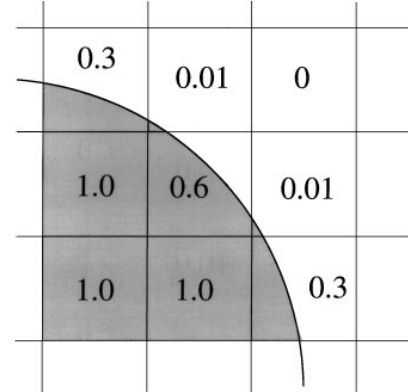
\includegraphics[width=0.5\textwidth]{plots/methodology/vof_basic.png} &
\hspace{-0.2cm}%
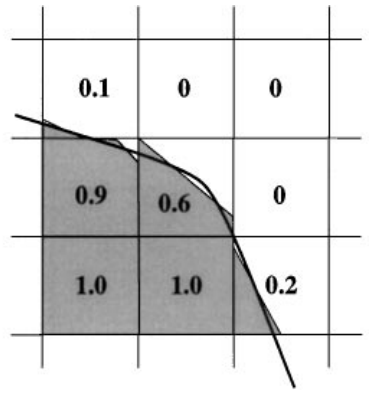
\includegraphics[width=0.473\textwidth]{plots/methodology/vof_plic.png} \\ 
\hspace{-0.2cm}%
(a) & (b) \\
\end{tabular}
\end{center}
\caption{ Exlicit definition of the interface location using the volume-of-fluid approach. 
These images are reproduced with permission from Scardovelli and Zaleski \cite{zaleskiannual}.
(a) The exact discrete representation of a circular arc on a regular Cartesian grid using the colour function field (volume fraction).
(b) The piecewise linear (PLIC) approximation to the smooth circular arc shown in (a), which entails second-order spatial accuracy.   
}
\label{vof_plic}
\end{figure}

\subsection*{Flux Computation}
Once the geometric PLIC reconstructions have been carried out, 
the interface segments are advected using the the velocity field. 
This entails computation of fluxes of the colour function, which 
can be computed via algebraic transport schemes (generally less accurate), 
or by using geometric reconstructions in either Eulerian, Lagrangian or hybrid frameworks.
In the context of our numerical platforms (`PARIS' and `Basilisk'), 
state-of-the-art \sidenote{The reader can refer to 
\cite{paris,basilisk} for further details}  
geometrical flux reconstruction procedues are utilised. 
The temporal integration of the fluxes could be carried out either as a 
series of one dimensional propagations along each of the spatial directions, 
termed as direction-split, or carried out in one single sweep, 
termed as multidimensional or unsplit.

Direction-split methods are more intuitive and easier to develop 
(extension of the one dimensional algorithm to 3D), 
but suffer from lack of conservation (to the order of 
machine precision) when it comes to 3D \sidenote{
A detailed exposition of this problem along with a noteworthy solution  
can be found in the work by Weymouth and Yue \cite{wy}}. 
Multidimensional (unsplit) methods have an advantage in that respect due to the 
fact that they are conservative by nature of their design, but are inherently 
more complicated to develop and implement, with no straightforward extension from 2D to 3D.    
For a more detailed and nuanced evaluation of the comparitive advantages of 
interfacial transport methods, we refer the reader to the recent review by 
Mirjalili et al. \cite{mirjalili2017interface} on the given subject.     
The propagation of the interface can be described by the evolution of
the colour function (volume fraction field) as  

\begin{align} 
	\frac{\partial C}{\partial t} + \boldsymbol{u} \cdot \nabla C = 0  	
\label{cvof_non}
\end{align}

We can express the left hand side of \eqref{cvof_non} in the conservative form as  

\begin{align} 
	\frac{\partial C}{\partial t} + \nabla \cdot \left(C \boldsymbol{u}\right) = C \left(\nabla \cdot \boldsymbol{u}\right) 	
\label{cvof_con}
\end{align}

As one can observe, the ``compression'' term on the right hand side of equation 
\ref{cvof_con} equals to zero in the context of incompressible flows without mass 
transfer, but it is important to keep this term in our numerical formulation within 
the direction-split framework. Discretization of the above equation results in :

\begin{align}
	C_{i,j,k}^{n,d+1} = C_{i,j,k}^{n,d} - F_{+}^{n,d}\left(C \right) - F_{-}^{n,d}\left(C \right) + \overline{C}_{i,j,k}^{n,d}\left(\frac{\Delta u_q}{\Delta x}\right)^{n,d}_{i,j,k}  
  \label{cvof_discrete}
\end{align}

The above equation represents an advection substep, the superscripts $n$ and $d$ refer to the timestep and 
direction of integration respectively. The notation $d=0$ refers to the field 
at the $n^{th}$ timestep, before any integration is performed along any direction. 
The fluxes $F_{\pm}^{n,d}(C)$ in equation \ref{cvof_discrete} are derived through geometrical reconstructions
\sidenote{For details regarding geometric flux reconstruction, refer to \cite{zaleskibook, zaleskiannual}}.
The $+$ and $-$ subcripts refer to the orientation with respect to the central cell ($i,j,k$).
The subscript $q$ refers to the direction corresponding to that given advection substep 
i.e either $X$, $Y$ or $Z$. In our case, our numerical platforms are based on cubic 
(regular Cartesian) grids, consequently there is no requirement for a subscript with $\Delta x$. 
After each substep, the interface is reconstructed once again with the updated 
volume fraction field in order to compute the fluxes for the next advection substep.  
Finally, the volume fraction field for the next timestep is given by 

\begin{align}
	 C^{n+1}_{i,j,k} = C^{n,3}_{i,j,k}  
\end{align}

The interpretation and numerical approximation of the prefactor $\overline{C}_{i,j,k}^{n,d}$ 
to the directional divergence, as well as the fluxes $F_{\pm}^{n,d}(C)$, depend 
on the exact nature of the geometrical advection scheme in question, 
which in our context is either CIAM (Lagrangian explicit) or Weymouth-Yue (Eulerian implicit) 
\sidenote{The classification of Lagrangian explicit and Eulerian implicit 
are in accordance with the paper by Aulisa et al. \cite{aulisa2003}}.
A brief outline of these two methods is presented in the subsequent sections.   

\paragraph{Lagrangian Explicit} 
This scheme was originally described in the work of Li \cite{li95}, `CIAM' being an 
abbreviation for the French title `\textit{Calcul d'interface affine par morceaux}', 
which can be thought of as a straightforward Lagrangian transport of the interface Heaviside function. 
After the interface segments are reconstructed from the discrete colour function 
at the start of the time-step, the interfacial points are transported by the component of the 
velocity field corresponding to the direction of transport. A geometrical interpretation of the scheme
is illustrated in figure \ref{fig:ciam}, reproduced from the seminal work of Gueyffier et al. \cite{gueyffier}. 

\begin{figure}[!h]
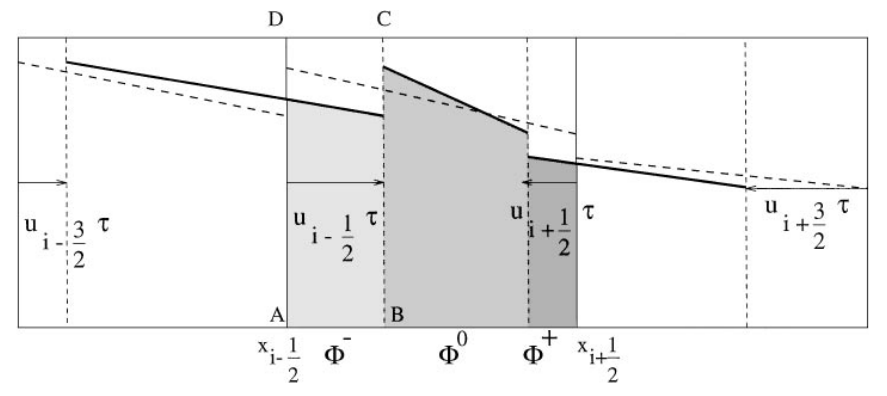
\includegraphics[width=1.0\textwidth]{plots/methodology/ciam.png} 
\caption{
Lagrangian transport of the interface segments using the CIAM scheme, the image
is reproduced with permission from Gueyffier et al. \cite{gueyffier}. 
A 2D schemetic of the geometric calculation of the fluxes of the volume 
fraction field is shown, for the advection substep along the horizontal direction.
The central cell ($i,j,k$) undergoes a net compression during this substep.
The fluxes $\Phi^{-}$ , $\Phi^{0}$ and $\Phi^{+}$ are the volumes under the 
advected interface segments advected by the interpolated velocity field,
intersected by the $(i,j,k)$ cell boundaries.
}
\label{fig:ciam}
\end{figure}

As one can infer from the geometrical representation in figure \ref{fig:ciam}, 
the fluxes $F_{\pm}^{n,d}(C)$ correspond to the volumes $\Phi^{-}$ and $\Phi^{+}$. 
Thus, the updated field $C_{i,j,k}^{n,d+1}$ is the sum of the 
three contributions $\Phi^{-}$ , $\Phi^{0}$ and $\Phi^{+}$. 
We can rewrite equation \ref{cvof_discrete} specifically for the CIAM scheme as   

\begin{align}
C_{i,j,k}^{n,d+1} =  C_{i,j,k}^{n,d}\left[1 + \left(\frac{\Delta u_q}{\Delta x}\right)^{n,d}_{i,j,k} \right] - F_{+}^{n,d}\left(C \right) - F_{-}^{n,d}\left(C \right)   
\label{ciam_discrete}
\end{align}

where the compression coefficient $\overline{C}_{i,j,k}^{n,d}$ is simply equal 
to the value of the colour function $C_{i,j,k}^{n,d}$ at the start of the 
corresponding advection substep. Although the flux terms cancel upon integration 
throughout the whole domain, one can clearly see that the compression terms do 
not sum up to zero due to the changing prefactor in front of the directional divergences. 
This precise issue brings us to the next advection scheme.      

\paragraph{Eulerian Implicit}
This advection scheme was developed by Weymouth and Yue \cite{wy} in order to 
specifically tackle the problem of discrete conservation when it comes to direction-split 
geometrical advection schemes \sidenote{By `discrete conservation' we mean that the sum of 
the directional divergences sum upto zero, to the accuracy of machine precision.}. 
The scheme fundamentally employs a forward Eulerian method in order to carry out temporal 
integration of the fluxes, with the fluxes themselves computed as the quantity of the substance 
entering or exiting a given control volume through its fixed surfaces, as shown in figure \ref{fig:wy}. 
This is in contrast with the flux computation method in the case of CIAM, 
where the interface segments are propagated forward in time in a Lagrangian fashion. 

\begin{figure}[!h]
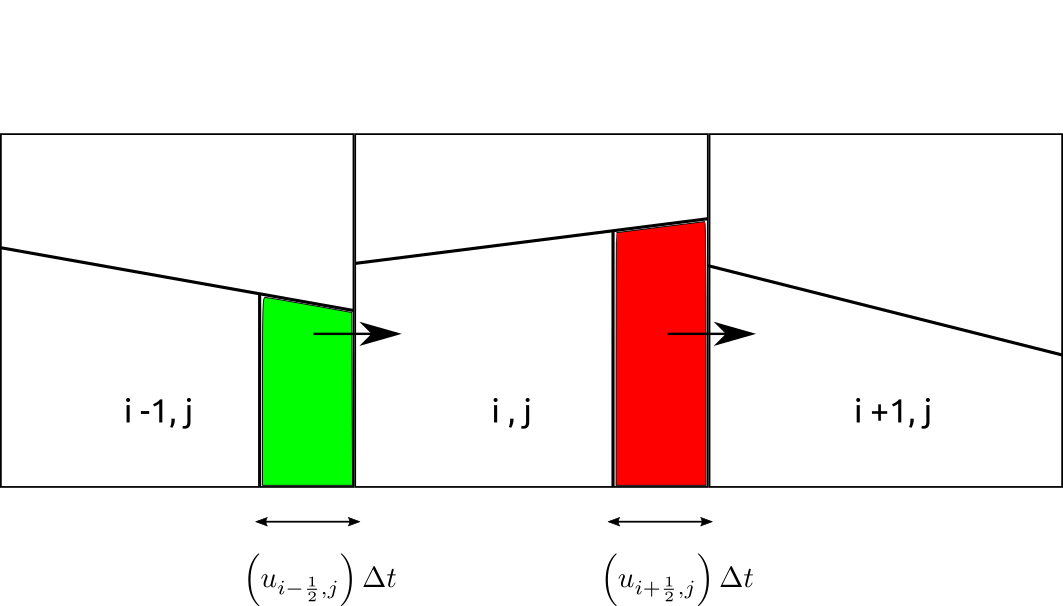
\includegraphics[width=1.0\textwidth]{plots/methodology/wy.png} 
\caption{ A 2D schemetic of the Eulerian (geometric) flux calculation  
using the Weymouth-Yue \cite{wy} scheme for the advection substep
along the horizontal direction, with the interface reconstructed 
using the volume fraction field at the start of the substep.
The colour fraction of the central cell ($i,j$) is updated during this substep
through the addition of the fluxes (coloured regions), with the green polygon corresponding
to the volume entering the cell $i,j$ from the $i-1,j$ and the red one corresponding to
that exiting $i,j$ into $i+1,j$. The geometric flux calculations are made on the basis
of the interfacial positions at the start of the substep, and the face centered velocities 
of the cell in question.}
\label{fig:wy}
\end{figure}

The subtle but important tactic used in this scheme lies in the manner in which the 
prefactor to the compression term \sidenote{Compression coefficient is used 
as a short-hand version of 'prefactor to the compression term'.}  is treated, with its definition being : 

\begin{align}
\overline{C}_{i,j,k}^{n,d} = H \left( C_{i,j,k}^{n,0} - 1/2 \right)
\label{wy_cond}
\end{align}

where $H$ is a one-dimensional Heaviside function. This renders the compression coefficient 
independent of the direction of the advection substep, consequently enabling the 
three discrete directional divergences to sum up to zero \sidenote{In numerical terms, we
can only ensure that they sum up to the accuracy of the Poisson solver $\sim 10^{-3} - 10^{-6}$
, with the limiting factor being the level of machine accuracy ($\sim 10^{-14} - 10^{-17}$). }
Therefore, the scheme is able to demonstrate volume conservation, subject to local 
CFL restrictions \sidenote{For a proof of discrete volume conservation subject to certain
CFL criteria, refer to the appendix of Weymouth and Yue \cite{wy}.}. To summarise, we can rewrite equation \ref{cvof_discrete}
for the Weymouth-Yue scheme as  

\begin{align}
C_{i,j,k}^{n,d+1} =  C \left[1 + \left(\frac{\Delta u_q}{\Delta x}\right)^{n,d}_{i,j,k} \right] - F_{+}^{n,d}\left(C \right) - F_{-}^{n,d}\left(C \right)   
\label{wy_discrete}
\end{align}

where $C$ is a constant with a value of either $0$ or $1$, determined by the value of $C_{i,j,k}^{n,0}$ according to equation \ref{wy_cond}.  

%---------------------------------------------------------------

\section{Time Marching}

In order to describe the overall numerical algorithm for the one-fluid Navier-Stokes equations with variable density and viscosity, we choose to the reframe our equations in a more convenient operator form, as presented below : 

\begin{align}
   \frac{\partial}{\partial t} \left( \rho \boldsymbol{u} \right) = L\left( \rho,\boldsymbol{u} \right) - \nabla p
\end{align}

The operator $L$ in the above expression can be decomposed as : 

\begin{align}
	L = L_{\textrm{adv}} + L_{\mu} + L_{\sigma} + L_{\textrm{g}} 
   \label{opr}
\end{align}

where the $L_{\textrm{adv}}$ represents the conservative advection, 
$L_{\mu}$ represents the diffusive forces generated by viscous stresses,
$L_{\sigma}$ represents the capillary forces arising from the surface tension model
and finally $L_{g}$ represents the volumetric (body forces) source term. 

\subsection*{Spatio-temporal Discretization}

We apply the spatially discretized versions of these operators (denoted by the superscript $h$) 
onto the primary variables ($C,\boldsymbol{u}$), and march forward in time using a small, 
possibly variable time-step $\tau$ such that $t_{n+1} = t_{n} + \tau$. 
We shall be dropping the subscripts $i,j,k$ from this point onwards, with the understanding 
that the operators in equation \ref{opr} apply uniformly to all control volumes. 
In the first part of the algorithm, the volume fraction field $C^{n}$ is updated to the next timestep 
, with the superscript $n$ signifying discretization in time. The operation can be written as follows        

\begin{align}
	C^{n+1} = C^{n} + \tau L^{h}_{\textrm{vof}}\left( C^{n},\boldsymbol{u}^{n}\right)  
\label{cvof_update}
\end{align}

The temporal evolution of the volume fraction field represented above by the 
operator $L^{h}_{\textrm{vof}}$ is in accordance with the Lagrangian explicit or Eulerian implicit 
advection schemes, as described in the previous sections. 
Once we have obtained the updated field $C^{n+1}$, we can move on to 
the temporal update of our momentum field given by 

\begin{align}
	\rho^{n+1}\cdot \boldsymbol{u}^{*} &= \rho^{n}\cdot \boldsymbol{u}^{n} + \tau L^{h}_{\textrm{adv}}\left( C^{n},\boldsymbol{u}^{n} \right) + \nonumber \\
				      & \tau \left[ L^{h}_{\mu}\left(C^{n+1},\boldsymbol{u}^{n}\right) + L^{h}_{\sigma}\left(C^{n+1}\right) + L^{h}_{\textrm{g}}\left(C^{n+1}\right)\right]
\label{mom_update}
\end{align}

In regions of constant density. the advection operator $L^{h}_{\textrm{adv}}$ 
is implemented using higher order spatial schemes 
coupled with a choice of non-linear flux limiters such as 
QUICK, ENO, WENO, Superbee, Verstappen and BCG.
\sidenote{These high-order spatial schemes are based on well established methods 
developed to deal with hyperbolic conservation laws, for more details refer to the 
studies of Leveque \cite{flim_1} and Sweby \cite{flim_2}.}. 
For control volumes in the vicinity of the interface location, we revert to lower order
schemes due to the sharp jumps in the material properties across the interface.  
The functionality of the operator $L^{h}_{\textrm{adv}}$ near the interface is tighly coupled
to that of $L^{h}_{\textrm{vof}}$ from equation \ref{cvof_update}, 
so as to ensure consistency in the discrete advection of mass and momentum.
The details regarding this coupling shall be the focus 
of subsequent chapters, where it is covered in more depth.

\subsection*{Pressure-Poisson Projection}

The velocity field is evolved using a classical time-splitting projection method 
as described in the seminal work of Chorin \cite{chorin1969convergence}, 
which involves predicting an `intermediate' velocity field $\boldsymbol{u}^{*}$ 
as given by equation \ref{mom_update}, followed by a correction step as follows        

\begin{align}
\boldsymbol{u}^{n+1} = \boldsymbol{u}^{*} - \frac{\tau}{\rho^{n+1}}\nabla^{h}p^{n+1}
\label{ufinal}
\end{align}

The discrete pressure field required to correct the intermediate velocity 
is determined by imposing the conservation of mass, which in our incompressible 
framework reduces to necessitating the resulting velocity field to be divergence-free (solenoidal)  

\begin{align}
\nabla^{h}\cdot\boldsymbol{u}^{n+1} = 0
\label{div}
\end{align}

Thus, combining equations \ref{ufinal} and \ref{div}, 
we are left with a variable coefficient Poisson equation for the pressure :  

\begin{align}
\nabla^{h}\cdot\left(\frac{\tau}{\rho^{n+1}}\nabla^{h}p^{n+1}\right) = \nabla^{h}\cdot \boldsymbol{u}^{*} 
	\label{poisson}
\end{align}

The Poisson solver used in `PARIS Simulator' to invert the elliptic operator 
appearing in eqn. \ref{poisson} is a red-black 
Gauss-Seidel (GS) solver with overrelaxation \sidecite{briggs1987}. 
There is also has an in-house implementation of a multigrid solver 
for structured grids with $2^{n}$ number of points per direction, 
utilizing a fully parallelized V-Cycle scheme \cite{briggs1987}. 
Relaxation operations are applied starting from the finest to the coarsest first, 
and then from the coarsest to the finest, with the number of relaxation operations 
being a user-adjustable parameter. Having a native multigrid solver allows 
for an efficient solution of the Poisson equation without the necessity
of having external libraries/pre-conditioners (e.g. HYPRE) installed on the system.
When it comes to `Basilisk', an atypical multigrid solver is implemented using 
a ``half'' V-cycle in order to deal with the spatial inhomogeity of the grid size
arising due to adaptive mesh refinement. 
For more details regarding the differences between the multigrid solver of `Basilisk'
and the classical implementation of a multigrid, one can refer to \sidecite{popinet_gerris}.


The whole set of operations described up to this point, 
constitutes a temporal integration scheme of the first-order, which can be expressed as 

\begin{align}
\left(C^{n+1},\boldsymbol{u}^{n+1}\right) = L_{1}\left( C^{n},\boldsymbol{u}^{n} \right)
\end{align}

where $L_{1}$ is the operator consisting of all the steps described 
so far, applied to the primary fields $C$ and $\boldsymbol{u}$. 
Therefore, a second-order time integration can easily be 
computed by using $L_{1}$ to get a first prediction    

\begin{align}
\left(C^{**},\boldsymbol{u}^{**}\right) = L_{1}\left( C^{n},\boldsymbol{u}^{n} \right)
\end{align}

The superscript $**$ refers to our first order prediction of the primary variables. 
Therefore, the second-order estimate can be obtained via averaging   

\begin{align}
\left(C^{n+1},\boldsymbol{u}^{n+1}\right) = \frac{1}{2}\left[ \left(C^{**},\boldsymbol{u}^{**} \right) + L_{1}\left( C^{**},\boldsymbol{u}^{**} \right) \right]
\end{align}

%---------------------------------------------------------------

\section{Source Terms}
The detailed descriptions of the methods used in our numerical platforms to deal with surface tension,
viscosity and body forces have already been carried out in \cite{paris, basilisk, popinet2009accurate}, 
therefore we briefly touch upon certain aspects of the operators in question, in particular, 
their interaction with the volume fraction field.

\subsection*{Surface Tension}
We use the Continuum Surface Force method (CSF) as our model for surface tension, 
coupled with height functions for curvature computation. 
The height functions used in our implementation were first introduced in \cite{popinet2009accurate}
, subsequently tested, revised and improved in \cite{bornia2011properties,owkes2015mesh}. 
In general, the height functions are used to compute the curvature field based 
on second-order finite differences applied to the heights. 
Although, in regions of poor interfacial resolution 
\sidenote{These are regions where the local radius of curvature is comparable to the grid size, in fact 
for certain cases the height functions perform poorly even for regions resolved by 10-20 grid points.}, 
the method reverts to certain fallbacks, one of which is curve fitting instead of height functions.  
The resulting curvature field is coupled with a well-balanced discretization with
respect to the discrete pressure gradient, with the same discretization 
stencil applied to the volumetric (body) force term as well. 


\subsection*{Viscous Diffusion}
We use second-order spatial discretizations of the viscous stresses, using centered differences
\sidenote{The exact implementation differs slightly between `Basilisk' and `PARIS Simulator'.}. 
The (variable) dynamic viscosity is computed based on the  
volume fraction field via weighted arithmetic or harmonic averaging (equations \ref{mu_chi}). 
The temporal treatment of the viscous term can be either in explicit or semi-implicit fashion,  
, but in the context of the present study we will be sticking exclusively with the explicit version.     

